\documentclass[10pt]{article}
\usepackage{mathtools}
\usepackage[margin=0.5cm]{geometry}

\title{Physics Formula Sheet}
\begin{document}
\textbf{\underline{Phox Physics Examples - SPH4U}}\\
\\
\textbf{\underline{Kinematics}} \\
\medskip
1. Iggy walks 9.0 km [N] and then 15 km [E $20^o$ S] and the entire trip takes 145 minutes.\\
Determine \\

a) Iggy's total displacement. 
b) Iggy's average velocity. \\

\medskip
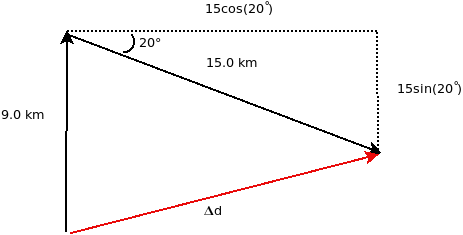
\includegraphics[scale=1]{Kinematics - 2D Displacement.png} \\




\end{document}